\documentclass[12pt,a4paper]{article}
\usepackage{tikz}
\usetikzlibrary{calc}
\begin{document}
\begin{figure}
\begin{center}
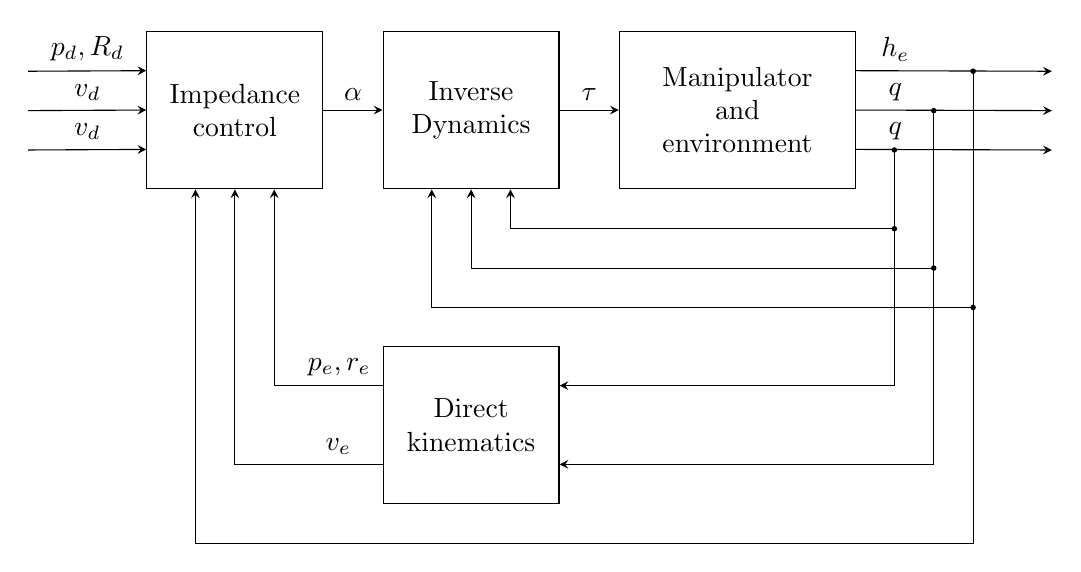
\begin{tikzpicture}[>=stealth]
  %coordinates
  \coordinate (orig)   at (0,0);
  \coordinate (LLD)    at (4,0);
  \coordinate (AroneA) at (-1/2,11/2);
  \coordinate (ArtwoA) at (-1/2,5);
  \coordinate (ArthrA) at (-1/2,9/2);
  \coordinate (LLA)    at (1,4);
  \coordinate (LLB)    at (4,4);
  \coordinate (LLC)    at (7,4);
  \coordinate (AroneC) at (25/2,11/2);
  \coordinate (ArtwoC) at (25/2,5);
  \coordinate (ArthrC) at (25/2,9/2);
  \coordinate (conCBD) at (21/2,9/2);
  \coordinate (conCB)  at (21/2,7/2);
  \coordinate (coCBD)  at (11,5);
  \coordinate (coCB)   at (11,3);
  \coordinate (conCBA) at (23/2,11/2);
  \coordinate (conCA)  at (23/2,5/2);

  %nodes
  \node[draw, minimum width=2cm, minimum height=2cm, anchor=south west, text width=2cm, align=center] (A) at (LLA) {Impedance\\control};
  \node[draw, minimum width=2cm, minimum height=2cm, anchor=south west, text width=2cm, align=center] (B) at (LLB) {Inverse\\Dynamics};
  \node[draw, minimum width=3cm, minimum height=2cm, anchor=south west, text width=2cm, align=center] (C) at (LLC) {Manipulator\\and\\environment};
  \node[draw, minimum width=2cm, minimum height=2cm, anchor=south west, text width=2cm, align=center] (D) at (LLD) {Direct\\kinematics};

  %edges
  \draw[->] (AroneA) -- node[above]{$p_d, R_d$} ($(A.180) + (0,1/2)$);
  \draw[->] (ArtwoA) -- node[above]{$v_d$} (A.180);
  \draw[->] (ArthrA) -- node[above]{$v_d$} ($(A.180) + (0,-1/2)$);

  \draw[->] (A.0) -- node[above] {$\alpha$} (B.180);
  \draw[->] (B.0) -- node[above] {$\tau$} (C.180);

  \draw[->] ($(C.0) + (0,1/2)$) -- node[above, pos=0.2]{$h_e$} (AroneC);
  \draw[->] (C.0) -- node[above, pos=0.2]{$q$} (ArtwoC);
  \draw[->] ($(C.0) + (0,-1/2)$) -- node[above, pos=0.2]{$q$} (ArthrC);

  \path[fill] (conCBD) circle[radius=1pt] (conCB) circle[radius=1pt];
  \path[draw,->] (conCBD) -- (conCB) -| ($(B.270) + (1/2,0)$);

  \path[fill] (coCBD) circle[radius=1pt] (coCB) circle[radius=1pt];
  \path[draw,->] (coCBD)  -- (coCB) -| (B.270);

  \path[fill] (conCBA) circle[radius=1pt] (conCA) circle[radius=1pt];
  \path[draw,->] (conCBA) -- (conCA) -| ($(B.270) + (-1/2,0)$);

  \path[draw,->] (conCB) |- ($(D.0) + (0,1/2)$);
  \path[draw,->] (coCB)  |- ($(D.0) + (0,-1/2)$);

  \path[draw,->] (conCA) |- ($(A.270) + (-1/2,0) + (0,-9/2)$) -- ($(A.270) + (-1/2,0)$);

  \path[draw,->] ($(D.180) + (0,1/2)$)  -| node[above,pos=0.2] {$p_e,r_e$} ($(A.270) + (1/2,0)$);
  \path[draw,->] ($(D.180) + (0,-1/2)$) -| node[above,pos=0.15] {$v_e$} (A.270);

\end{tikzpicture}

\end{center}

\end{figure}
\end{document}